\chapter{Background}

This chapter covers the foundational knowledge you need to understand our work. We start with the mathematical and computational preliminaries. Then we review the existing literature on ANN-based ODE solvers and similar applications. We identify the research gaps that motivate our study. Finally, we wrap up with a brief summary.

\section{Preliminaries}

This section provides the necessary background knowledge to understand the rest of the report.

\subsection{Ordinary Differential Equations}

An ODE describes how a quantity changes with respect to a single independent variable. A general first-order ODE takes the form:

\begin{equation}
\frac{dy}{dt} = f(t, y), \quad y(t_0) = y_0
\label{eq:first_order_ode}
\end{equation}

where $y(t)$ is the unknown function, $t$ is the independent variable, and $y_0$ is the initial condition.

\subsection{The Lorenz-1960 System}

The Lorenz-1960 system \cite{lorenz1960max} consists of three coupled nonlinear ODEs for meteorological modeling. We target the formulation from \cite{matthews2024pinnde} (Section 4.2):

\begin{equation}
\begin{aligned}
\frac{dx}{dt} &= kl\left(\frac{1}{k^2 + l^2} - \frac{1}{k^2}\right) yz \\
\frac{dy}{dt} &= kl\left(\frac{1}{l^2} - \frac{1}{k^2 + l^2}\right) xz \\
\frac{dz}{dt} &= \frac{kl^2}{2}\left(\frac{1}{k^2} - \frac{1}{l^2}\right) xy
\end{aligned}
\label{eq:lorenz1960}
\end{equation}

with $k = 2$, $l = 1$, initial conditions $x(0) = 0.5$, $y(0) = 0.75$, $z(0) = 1$, and $t \in [0, 1]$. Its nonlinear, coupled dynamics make it an excellent benchmark for numerical solvers.

\subsection{Classical Numerical Methods}

Euler's method approximates the solution via a first-order Taylor expansion:
\begin{equation}
y_{n+1} = y_n + h \cdot f(t_n, y_n)
\end{equation}
where $h$ is the step size. It is simple but accumulates errors quickly.

The fourth-order Runge-Kutta method (RK4) evaluates the derivative at multiple points per step for higher accuracy:
\begin{equation}
y_{n+1} = y_n + \frac{h}{6}(k_1 + 2k_2 + 2k_3 + k_4)
\end{equation}

Both methods are mesh-dependent, require re-solving for every new initial condition, and struggle with stiff equations.

\subsection{Artificial Neural Networks}

A feedforward ANN (Multilayer Perceptron) consists of an input layer, hidden layers, and an output layer. Each neuron computes:

\begin{equation}
a_i(\mathbf{x}) = \sigma\left(\mathbf{w}^{(i)} \cdot \mathbf{x} + b^{(i)}\right)
\label{eq:neuron}
\end{equation}

where $\mathbf{w}^{(i)}$ are weights, $b^{(i)}$ is bias, and $\sigma$ is an activation function \cite{lau2020oden}. The Universal Approximation Theorem \cite{lau2020oden, babni2025error, hornik1989multilayer} guarantees that a network with at least one hidden layer can approximate any continuous function to arbitrary accuracy. Common activation functions include:
\begin{itemize}
    \item \textbf{Sigmoid}: $\sigma(x) = \frac{1}{1 + e^{-x}}$, maps inputs to $(0, 1)$
    \item \textbf{Tanh}: $\sigma(x) = \frac{e^x - e^{-x}}{e^x + e^{-x}}$, maps inputs to $(-1, 1)$
    \item \textbf{ReLU}: $\sigma(x) = \max(0, x)$, efficient but non-smooth at zero
    \item \textbf{GELU/Swish}: smooth ReLU approximations with better gradient flow
\end{itemize}

Training minimizes a loss function $L(\theta)$ over network parameters $\theta$ using gradient descent. Backpropagation computes gradients via the chain rule, and optimizers like Adam adapt learning rates per parameter \cite{dubey2024solving, audu2026neural}.

\subsection{ANN-Based ODE Solving}

Instead of stepping through the domain, ANNs learn a continuous solution function over the entire domain. The standard approach \cite{lagaris1998ann, mall2013comparison, okereke2021novel} constructs a trial solution:

\begin{equation}
\psi_t(x, \mathbf{p}) = A(x) + F(x, N(x, \mathbf{p}))
\label{eq:trial_solution}
\end{equation}

where $A(x)$ satisfies the initial/boundary conditions exactly, and $N(x, \mathbf{p})$ is the neural network output. The loss function measures how well this trial solution satisfies the ODE:

\begin{equation}
L(\mathbf{p}) = \frac{1}{N} \sum_{i=1}^{N} \left[ \frac{d\psi_t(x_i, \mathbf{p})}{dx} - f(x_i, \psi_t(x_i, \mathbf{p})) \right]^2
\label{eq:ode_loss}
\end{equation}

Minimizing this loss yields a differentiable, closed-form approximate solution without requiring knowledge of the exact answer.

\subsection{Physics-Informed Neural Networks}

PINNs embed governing equations directly into the loss function \cite{raissi2019pinn, matthews2024pinnde, babni2025error, audu2026neural}:

\begin{equation}
L(\theta) = L_{\text{data}} + \lambda_1 L_{\text{physics}} + \lambda_2 L_{\text{IC/BC}}
\end{equation}

The physics loss uses automatic differentiation to compute derivatives of the network output. This enables training with sparse or no data, but balancing the loss terms requires careful hyperparameter tuning.

\subsection{Network Architectures}

To better understand the differences in methodology, we present the standard architectures used in recent studies. Figure~\ref{fig:ann_arch} illustrates a typical Artificial Neural Network (ANN) architecture used for predicting system parameters without physics-informed constraints \cite{Bre}. This standard feedforward structure relies entirely on data-driven learning through backpropagation.

\begin{figure}[H]
    \centering
    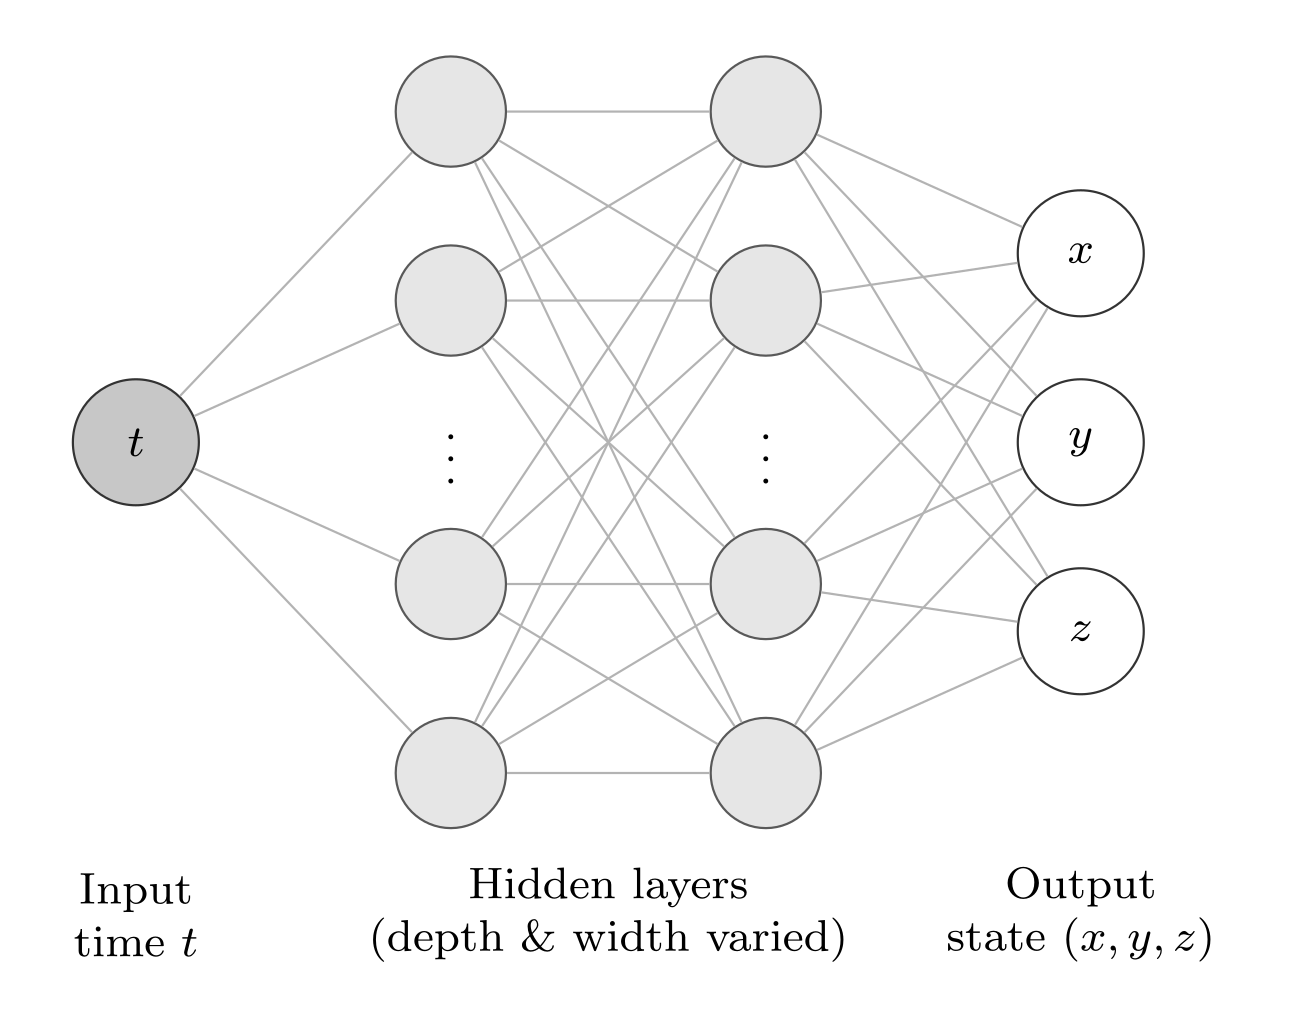
\includegraphics[width=0.85\textwidth]{ann_architecture.png}
    \caption{Typical Artificial Neural Network architecture \cite{Bre}.}
    \label{fig:ann_arch}
\end{figure}

In contrast, Figure~\ref{fig:pinn_arch} demonstrates a Physics-Informed Neural Network (PINN) architecture. In this approach, the standard ANN output is further constrained by physical laws---specifically, the governing differential equations of the system---which are embedded directly into the loss function \cite{Zhai}.

\begin{figure}[H]
    \centering
    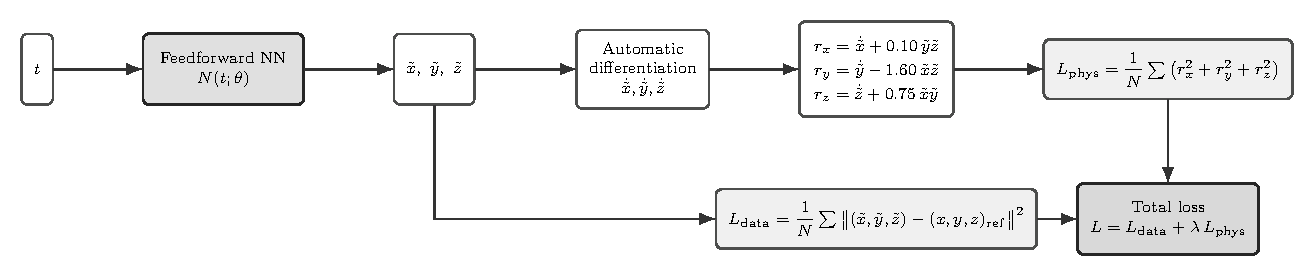
\includegraphics[width=\textwidth]{pinn_architecture.pdf}
    \caption{Architecture of a Physics-Informed Neural Network incorporating physical loss \cite{Zhai}.}
    \label{fig:pinn_arch}
\end{figure}


\section{Literature Review}

\subsection{Similar Applications}

Dubey et al. \cite{dubey2024solving} used an ANN (tanh activation) to solve coupled first-order ODEs with an error of $2.88 \times 10^{-3}$ in a maximum of 120 iterations. A comparable PyTorch-based ANN was used by Audu et al. \cite{audu2024utilizing}, which converged in 200--1500 iterations. Okereke et al. \cite{okereke2021novel} bypassed backpropagation by calculating the weights based on regression with Gaussian Radial Basis Functions. The ODEN framework developed by Lau and Werth \cite{lau2020oden} demonstrates that NNs outperform RK4 on rapidly oscillating solutions, with errors of $\sim 10^{-4}$. On a damped vibration equation, Mall and Chakraverty \cite{mall2013comparison} compared arbitrary versus regression-based weight initialization and they found that regression-based weights reduce maximum deviation from 3.67\% to 1.47\%. Murugesh et al. \cite{murugesh2025novel} used neural networks with block numerical methods to directly solve higher-order ODEs and obtaining errors near machine precision ($\sim 10^{-10}$). Pratama et al. \cite{pratama2022ann} surveyed three ANN-based PDE solvers (PyDEns, NeuroDiffEq, Nangs) and used 3 hidden layers with 32 neurons and tanh activation. NeuroDiffEq uses the Trial Approximate Solution methodology, which suggests that initial conditions are hardcoded in the ansatz. This is a pure ANN method that is applied to our research.


\subsection{Related Research}

\subsubsection{Physics-Informed Approaches}

PinnDE was proposed by Matthews and Bihlo \cite{matthews2024pinnde}, which solved the Lorenz-1960 system using a DeepONet (4 hidden layers, 40 nodes, tanh, Adam optimizer). Their DeepONet is trained to learn the operator $G(u_0)(t, x)$ which provides solutions given initial conditions over $[0, 1]$. This is the closest baseline to our target problem, but it relies on physics-informed loss terms. Babni et al. \cite{babni2025error} generalized the trial construction $\tilde{u}(x, \theta) = P(x) + Q(x)N(x, \theta)$ by replacing $Q(x)$ with a flexible $\varphi(x)$, proving the error bound $|N_\varphi(t, \theta) - u(t)| \leq e^{\kappa|t - t_0|} L_\varphi(\theta)$. This verifies that the smaller the loss, the smaller the solution error. Audu et al. \cite{audu2026neural} compared PINN and ANN models using six first-order ODE tests. Their PINN had an error of $10^{-8}$ to $10^{-10}$ which was much better as compared to ANN. This raises the issue of whether architecture optimization can bridge this gap or not.

\subsubsection{Pure ANN Approaches}

The NeuroDiffEq Trial Approximate Solution is physics-free. Pratama et al. \cite{pratama2022ann} found that NeuroDiffEq can train without physics loss terms which is consistent with our methodology. But they benchmarked only on the heat equation which is linear. Dubey et al. \cite{dubey2024solving} claim that plain ANNs can solve coupled ODEs but used a fixed architecture. Okereke et al. \cite{okereke2021novel} removed backpropagation through weight computation instead of polynomial fitting. Audu et al. \cite{audu2024utilizing} achieved an error of $10^{-4}$ with a sigmoid ANN on three first-order ODEs. All these studies do not examine the implications of building patterns on performance.

\subsubsection{Architecture and Loss Function Studies}

Mall and Chakraverty \cite{mall2013comparison} made comparisons between 4, 5, and 6 hidden nodes with random and regression-based weights. Weights that are based on regression are always better compared to random weights. After 6 nodes they found that accuracy remains the same. They applied only sigmoid activation on simple ODEs. Lau and Werth \cite{lau2020oden} discovered that sigmoid / tanh need less training in comparison to ReLU / ELU. Xavier initialization speeds up the convergence and Adam is better than SGD. They did not vary systematically depth and width. Xiong \cite{xiong2022new} arranged seven constructions (polynomial, exponential, hyperbolic, logarithmic, logistic, sigmoid, softplus) of loss functions. Exponential is best when applied to the law of Newton cooling and logarithmic is best when it is applied to the motor suspension system.

\subsubsection{Lorenz System Studies}

Aslam et al. \cite{aslam2024neuro} have used ANN + PSO-NNA hybrid optimization to solve Lorenz equations (Neurons=10, sigmoid, N=90, independent runs=100). They are directed to a diverse Lorenz parameterization ($\sigma, \rho, \beta$), are based on meta heuristic optimization and do not compare architectures.

\subsubsection{Neural ODEs}

Chen et al. \cite{chen2018neural} proposed neural ODEs where the derivative function $\frac{dh(t)}{dt} = f(h(t), t, \theta)$ that is parameterized with a neural network and trained using the adjoint method efficient for backpropagation. This sample is quite different than ours where we learn the dynamics ($f$) while neural ODEs find the approximation of the solution ($y(t)$) itself.

\subsubsection{Hybrid Approaches}

Murugesh et al. \cite{murugesh2025novel} proposed a Neural-ODE Hybrid Block Method with the update rule:

\begin{equation}
y(t_{k+1}) = y(t_k) + h \sum_{j=0}^{m-1} \omega_j f_\theta(t_{k-j}, y_{k-j}) + \sum_{i=0}^{m-1} \alpha_i F(t_{k-i}, y_{k-i})
\end{equation}

where $\omega_j$ and $\alpha_j$ balance neural versus numerical contributions. It achieved machine-precision errors on harmonic oscillators and the Van der Pol equation.

\clearpage % Ensures we start at the top of a fresh page so we have maximum room

\section{Gap Analysis}

Table~\ref{tab:gap_analysis_updated} summarizes what each reviewed paper covers and where gaps exist.

\vspace{-1em} % Pulls the table up slightly closer to the text

\begin{table}[!ht] % Using !ht is safer and won't crash your document
    \centering
    \caption{Comprehensive Literature Gap Analysis}
    \label{tab:gap_analysis_updated}
    \tiny % Using \tiny ensures the table is physically short enough to share the page with your list
    \renewcommand{\arraystretch}{1.0} 
    \setlength{\tabcolsep}{2pt} % Shrinks padding to fit text better
    
    \begin{tabularx}{\textwidth}{| 
        >{\hsize=0.6\hsize\raggedright\arraybackslash}X | 
        >{\hsize=1.15\hsize\raggedright\arraybackslash}X | 
        >{\hsize=1.15\hsize\raggedright\arraybackslash}X | 
        >{\hsize=1.05\hsize\raggedright\arraybackslash}X | 
        >{\hsize=1.05\hsize\raggedright\arraybackslash}X | 
        >{\hsize=1.0\hsize\raggedright\arraybackslash}X |
        }
        \hline
        \textbf{Paper} & \textbf{Methodological Approach} & \textbf{Target Differential Equations} & \textbf{Architectural Investigation} & \textbf{Lorenz-1960 Application} & \textbf{Plain ANN Implementation} \\
        \hline
        
        \cite{matthews2024pinnde} & PINN + DeepONet: Integrates physics laws and operator networks into the loss function. & Solves both ODEs and PDEs using governing physics. & No systematic study of network structural impact. & Evaluated specifically as a complex dynamical system. & Uses physics-informed logic, not a plain ANN. \\
        \hline
        
        \cite{pratama2022ann} & PyDEns / ANN: Standard networks for field estimation. & Primary focus on solving Partial Differential Equations (PDEs). & General overview without specific layer/neuron testing. & The study does not address the Lorenz model. & Covers standard ANN architectures for PDEs. \\
        \hline
        
        \cite{chen2018neural} & Neural ODE: Derivative represented as a neural network. & Models continuous-time dynamics for ODEs. & Focuses on functional flexibility, not structural depth. & Not specifically tested on the Lorenz system. & Relies on specialized ODE-solver integration. \\
        \hline
        
        \cite{aslam2024neuro} & ANN + PSO-NNA: ANN with Particle Swarm Optimization. & Applied to solving Ordinary Differential Equations. & Optimization focuses on weights, not architectural depth. & Directly applied to Lorenz-based chaotic dynamics. & Uses heuristic optimization instead of plain training. \\
        \hline
        
        \cite{lau2020oden} & Plain ANN: Standard feedforward network approach. & General application for approximating ODE solutions. & Provides a limited (partial) study on hidden layers. & Tested on other benchmarks, not Lorenz-1960. & Utilizes a standard, plain ANN configuration. \\
        \hline
        
        \cite{mall2013comparison} & ANN: Implementation of neural networks for equations. & Targets solutions for ODEs in engineering. & Includes a detailed study on network architecture. & Application restricted to simpler, non-chaotic ODEs. & Employs a basic feedforward ANN structure. \\
        \hline
        
        \cite{xiong2022new} & ANN: Simple neural solver for dynamic systems. & Focused on solving Ordinary Differential Equations. & Does not explore the impact of different layer counts. & Does not address the chaotic Lorenz-1960 model. & Uses a traditional, data-driven ANN model. \\
        \hline
        
        \cite{babni2025error} & PINN: Physics-Informed Neural Networks approach. & Solves ODEs by embedding equations in the loss function. & No investigation into depth or width performance. & Not applied to the meteorological Lorenz model. & Strictly uses physics-informed constraints. \\
        \hline
        
        \cite{dubey2024solving} & Plain ANN: Feedforward network trained on numerical data. & Applied to various Ordinary Differential Equations. & Lacks a systematic study of network architecture. & No specific testing on the Lorenz system. & Uses a standard numerical data training pipeline. \\
        \hline
        
        \cite{okereke2021novel} & ANN: Basic neural network models for ODEs. & Aimed at solving standard ODE systems. & Does not perform structural performance analysis. & No mention or testing of the Lorenz-1960 system. & Follows a traditional, plain ANN approach. \\
        \hline
        
        \cite{audu2024utilizing} & Plain ANN: Usage for initial value problems in ODEs. & Specifically handles ODE solution approximation. & No detailed evaluation of layers or neurons. & Focused on other common types of ODEs. & Relies on a standard feedforward structure. \\
        \hline
        
        \cite{audu2026neural} & PINN vs ANN: A comparative study of two methods. & Analysis restricted to Ordinary Differential Equations. & Lacks an in-depth architecture comparison study. & Not applied to the Lorenz-1960 model. & Discusses ANN only in comparison to PINN. \\
        \hline
        
        \cite{murugesh2025novel} & Hybrid: Combines different neural modeling techniques. & Solves ODEs using integrated hybrid approaches. & Architecture optimization is not the primary focus. & Does not utilize the Lorenz-1960 test case. & Incorporates external optimization methods. \\
        \hline

        \cite{lagaris1998ann} & ANN: Trial-solution method using a feedforward network. & Solves ODEs, ODE systems, and PDEs. & No systematic study of layers or neurons. & Does not test the Lorenz-1960 system. & Plain feedforward ANN trained on the ODE residual. \\
        \hline

        \cite{raissi2019pinn} & PINN: Embeds governing equations in the loss function. & Targets forward and inverse nonlinear PDEs. & No systematic study of depth or width. & Not applied to the Lorenz-1960 model. & Uses physics-informed constraints, not a plain ANN. \\
        \hline

        \cite{lorenz1960max} & Analytical: Reduces the vorticity equation to three ODEs. & Derives the coupled nonlinear Lorenz-1960 ODEs. & Predates neural network architecture studies. & Defines the original Lorenz-1960 system. & Uses no neural network of any kind. \\
        \hline

        \cite{hornik1989multilayer} & Theory: Proves the universal approximation property. & Not concerned with differential equations. & Shows one hidden layer suffices for approximation. & Does not address the Lorenz-1960 system. & Covers feedforward networks in general, not a solver. \\
        \hline

        \textbf{Our Work} & \textbf{Plain ANN: Traditional feedforward network.} & \textbf{Direct solution of coupled ODE systems.} & \textbf{Comprehensive study of hidden layers and density.} & \textbf{Primary test case for predicting chaotic dynamics.} & \textbf{Purely data-driven ANN without physics aids.} \\
        \hline
        
    \end{tabularx}
\end{table}

The literature review reveals five specific gaps that our research addresses:

\begin{enumerate}
    \item \textbf{No architecture study for the Lorenz-1960 system:} Matthews and Bihlo \cite{matthews2024pinnde} solve the Lorenz-1960 system but use a fixed DeepONet architecture without optimization. Aslam et al. \cite{aslam2024neuro} study a different Lorenz parameterization. No existing paper systematically compares ANN architectures on the Lorenz-1960 system.

    \item \textbf{No PINN vs. plain ANN comparison on Lorenz-1960:} Audu et al. \cite{audu2026neural} compared PINN and ANN on simple first-order ODEs. No study makes this comparison on a nonlinear, coupled ODE system like Lorenz-1960.

    \item \textbf{No systematic activation function study for ODE solving:} Pratama et al. \cite{pratama2022ann} use tanh throughout without ablation. Lau and Werth \cite{lau2020oden} note that sigmoid and tanh outperform ReLU but do not test modern alternatives like GELU or Swish. Mall and Chakraverty \cite{mall2013comparison} use only sigmoid. No study compares activation functions (tanh, ReLU, sigmoid, GELU, Swish) on a coupled ODE system.

    \item \textbf{No systematic depth and width study for ODE solution quality:} Mall and Chakraverty \cite{mall2013comparison} test 4, 5, and 6 nodes on simple ODEs. Lau and Werth \cite{lau2020oden} observe that architecture should match equation complexity. But no paper systematically varies both depth (2--6 layers) and width (20--100 neurons) to find the optimal configuration for a Lorenz-type system.

    \item \textbf{Limited generalization studies:} Most papers train for a single initial condition. The ability to generalize across different initial conditions remains largely unexplored for coupled nonlinear ODE systems.
\end{enumerate}

Our research fills these gaps by performing a systematic architecture comparison on the Lorenz-1960 ODE system using plain ANNs. We vary depth, width, and activation functions while benchmarking against RK4 reference solutions and the PINN-based results from Matthews and Bihlo \cite{matthews2024pinnde}.


\section{Summary}

This chapter established the necessary background for our research. We reviewed the mathematical foundations of ODEs, the Lorenz-1960 system, classical numerical methods, and ANN-based solving approaches. The literature review covered 17 research papers spanning physics-informed methods, pure ANN approaches, architecture studies, Lorenz system solvers, Neural ODEs, and hybrid techniques.

The gap analysis reveals that no existing study performs a systematic architecture comparison of plain ANNs on the Lorenz-1960 ODE system. Existing works either use fixed architectures, focus on simpler equations, or rely on physics-informed loss terms. Our research directly addresses this gap by varying network depth, width, and activation functions to identify the optimal ANN architecture for solving the Lorenz-1960 system as an initial value problem.

The next chapter presents our project design, including the detailed methodology, experimental setup, and evaluation plan.

